% Options for packages loaded elsewhere
\PassOptionsToPackage{unicode}{hyperref}
\PassOptionsToPackage{hyphens}{url}
%
\documentclass[
]{article}
\usepackage{amsmath,amssymb}
\usepackage{iftex}
\ifPDFTeX
  \usepackage[T1]{fontenc}
  \usepackage[utf8]{inputenc}
  \usepackage{textcomp} % provide euro and other symbols
\else % if luatex or xetex
  \usepackage{unicode-math} % this also loads fontspec
  \defaultfontfeatures{Scale=MatchLowercase}
  \defaultfontfeatures[\rmfamily]{Ligatures=TeX,Scale=1}
\fi
\usepackage{lmodern}
\ifPDFTeX\else
  % xetex/luatex font selection
\fi
% Use upquote if available, for straight quotes in verbatim environments
\IfFileExists{upquote.sty}{\usepackage{upquote}}{}
\IfFileExists{microtype.sty}{% use microtype if available
  \usepackage[]{microtype}
  \UseMicrotypeSet[protrusion]{basicmath} % disable protrusion for tt fonts
}{}
\makeatletter
\@ifundefined{KOMAClassName}{% if non-KOMA class
  \IfFileExists{parskip.sty}{%
    \usepackage{parskip}
  }{% else
    \setlength{\parindent}{0pt}
    \setlength{\parskip}{6pt plus 2pt minus 1pt}}
}{% if KOMA class
  \KOMAoptions{parskip=half}}
\makeatother
\usepackage{xcolor}
\usepackage[margin=1in]{geometry}
\usepackage{graphicx}
\makeatletter
\def\maxwidth{\ifdim\Gin@nat@width>\linewidth\linewidth\else\Gin@nat@width\fi}
\def\maxheight{\ifdim\Gin@nat@height>\textheight\textheight\else\Gin@nat@height\fi}
\makeatother
% Scale images if necessary, so that they will not overflow the page
% margins by default, and it is still possible to overwrite the defaults
% using explicit options in \includegraphics[width, height, ...]{}
\setkeys{Gin}{width=\maxwidth,height=\maxheight,keepaspectratio}
% Set default figure placement to htbp
\makeatletter
\def\fps@figure{htbp}
\makeatother
\setlength{\emergencystretch}{3em} % prevent overfull lines
\providecommand{\tightlist}{%
  \setlength{\itemsep}{0pt}\setlength{\parskip}{0pt}}
\setcounter{secnumdepth}{-\maxdimen} % remove section numbering
\usepackage[english]{babel}
\usepackage{tcolorbox}
\usepackage{enumitem}
\usepackage{gensymb}
\usepackage{booktabs}
\ifLuaTeX
  \usepackage{selnolig}  % disable illegal ligatures
\fi
\usepackage{bookmark}
\IfFileExists{xurl.sty}{\usepackage{xurl}}{} % add URL line breaks if available
\urlstyle{same}
\hypersetup{
  pdftitle={Description and choice data for the domain ``Surface area''},
  hidelinks,
  pdfcreator={LaTeX via pandoc}}

\title{Description and choice data for the domain ``Surface area''}
\author{}
\date{\vspace{-2.5em}}

\begin{document}
\maketitle

\graphicspath{
  {../experiment/figures/}       % figures used in experiment
}

\subsection{\texorpdfstring{Description of the choice domain 21,
\texttt{Surface\ area}}{Description of the choice domain 21, Surface area}}\label{description-of-the-choice-domain-21-surface-area}

The prompt question and the universe of five response options in the
choice domain \texttt{Surface\ area} are as follows. The labels \(a\),
\(b\), \(c\), \(d\) and \(e\) were not displayed during the experiment
and are indicated here to allow cross-referencing with data tables and
visualizations below and results in the paper.

\% Surface area

These countries are ranked, respectively, 2nd through 6th in terms of
surface area, including inland bodies of water. In millions of square
kilometres, those surface areas are 9.984, 9.573, 9.525, 8.516 and
7.692.

\begin{tcolorbox}
Which one of the following countries do you think has the greatest surface area, including inland bodies of water?
    
\begin{itemize}
    \setlength\itemsep{-5pt}
    \item Canada
    \item United States of America
    \item China
    \item Brazil
    \item Australia
\end{itemize}
\end{tcolorbox}

The following figure is a screenshot from the actual experiment, with
one of the 26 possible menus for this domain.

\begin{figure}
\centering
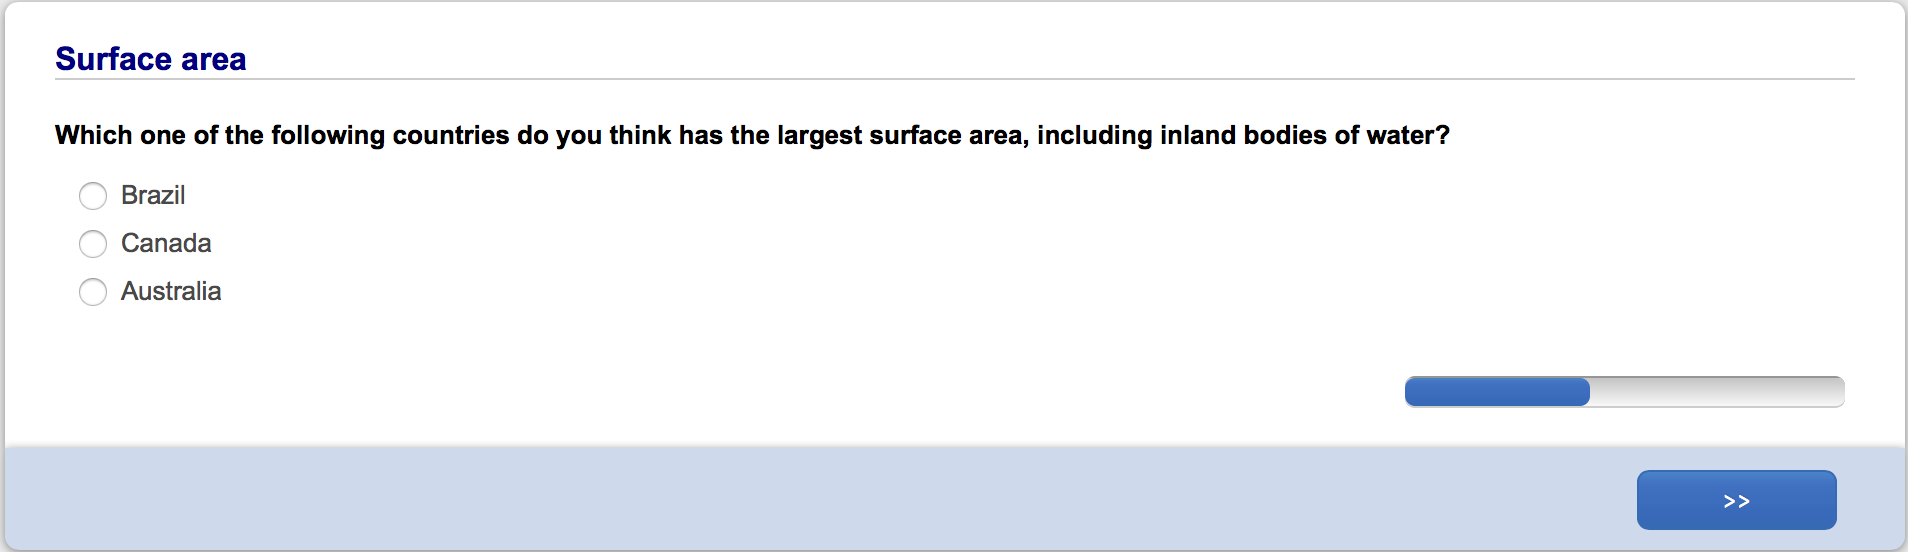
\includegraphics{/Users/williammccausland/Git_repos/Population/experiment/screenshots/screenshot_surface_area.png}
\caption{Screenshot for domain Surface area}
\end{figure}

\pagebreak

\subsection{Choice data for domain 21, Surface
area}\label{choice-data-for-domain-21-surface-area}

Table \ref{t:count_prop} shows choice counts and choice proportions for
this choice domain. For each menu \(A\) and each object
\(x \in \{a,b,c,d,e\}\), \(N_A(x)\) is the number of participants who
chose object \(x\) from menu \(A\) and \(\hat P_A(x)\) is the
corresponding proportion of participants who chose \(x\) from \(A\).
When \(x \notin A\), a dash is displayed.

\begin{table}\centering

\begin{tabular}{lrrrrrrrrrr}
\toprule
\multicolumn{1}{c}{ } & \multicolumn{5}{c}{Choice counts} & \multicolumn{5}{c}{Choice proportions} \\
\cmidrule(l{3pt}r{3pt}){2-6} \cmidrule(l{3pt}r{3pt}){7-11}
Menu $A$ & $N_A(a)$ & $N_A(b)$ & $N_A(c)$ & $N_A(d)$ & $N_A(e)$ & $\hat P_A(a)$ & $\hat P_A(b)$ & $\hat P_A(c)$ & $\hat P_A(d)$ & $\hat P_A(e)$\\
\midrule
$\{a,b\}$ & 37 & 3 & - & - & - & 0.925 & 0.075 & - & - & -\\
$\{a,c\}$ & 38 & - & 2 & - & - & 0.950 & - & 0.050 & - & -\\
$\{b,c\}$ & - & 24 & 16 & - & - & - & 0.600 & 0.400 & - & -\\
$\{a,b,c\}$ & 31 & 5 & 4 & - & - & 0.775 & 0.125 & 0.100 & - & -\\
$\{a,d\}$ & 40 & - & - & 1 & - & 0.976 & - & - & 0.024 & -\\
\addlinespace
$\{b,d\}$ & - & 30 & - & 11 & - & - & 0.732 & - & 0.268 & -\\
$\{a,b,d\}$ & 31 & 9 & - & 0 & - & 0.775 & 0.225 & - & 0.000 & -\\
$\{c,d\}$ & - & - & 23 & 17 & - & - & - & 0.575 & 0.425 & -\\
$\{a,c,d\}$ & 34 & - & 5 & 1 & - & 0.850 & - & 0.125 & 0.025 & -\\
$\{b,c,d\}$ & - & 23 & 13 & 4 & - & - & 0.575 & 0.325 & 0.100 & -\\
\addlinespace
$\{a,b,c,d\}$ & 30 & 3 & 5 & 2 & - & 0.750 & 0.075 & 0.125 & 0.050 & -\\
$\{a,e\}$ & 38 & - & - & - & 2 & 0.950 & - & - & - & 0.050\\
$\{b,e\}$ & - & 24 & - & - & 16 & - & 0.600 & - & - & 0.400\\
$\{a,b,e\}$ & 35 & 3 & - & - & 2 & 0.875 & 0.075 & - & - & 0.050\\
$\{c,e\}$ & - & - & 23 & - & 17 & - & - & 0.575 & - & 0.425\\
\addlinespace
$\{a,c,e\}$ & 34 & - & 3 & - & 3 & 0.850 & - & 0.075 & - & 0.075\\
$\{b,c,e\}$ & - & 20 & 12 & - & 8 & - & 0.500 & 0.300 & - & 0.200\\
$\{a,b,c,e\}$ & 27 & 7 & 4 & - & 2 & 0.675 & 0.175 & 0.100 & - & 0.050\\
$\{d,e\}$ & - & - & - & 14 & 26 & - & - & - & 0.350 & 0.650\\
$\{a,d,e\}$ & 36 & - & - & 0 & 4 & 0.900 & - & - & 0.000 & 0.100\\
\addlinespace
$\{b,d,e\}$ & - & 21 & - & 4 & 15 & - & 0.525 & - & 0.100 & 0.375\\
$\{a,b,d,e\}$ & 27 & 5 & - & 2 & 6 & 0.675 & 0.125 & - & 0.050 & 0.150\\
$\{c,d,e\}$ & - & - & 25 & 3 & 12 & - & - & 0.625 & 0.075 & 0.300\\
$\{a,c,d,e\}$ & 34 & - & 5 & 0 & 1 & 0.850 & - & 0.125 & 0.000 & 0.025\\
$\{b,c,d,e\}$ & - & 12 & 17 & 3 & 8 & - & 0.300 & 0.425 & 0.075 & 0.200\\
\addlinespace
$\{a,b,c,d,e\}$ & 26 & 5 & 6 & 0 & 3 & 0.650 & 0.125 & 0.150 & 0.000 & 0.075\\
\bottomrule
\end{tabular}
\caption{Observed choice counts and proportions.}
\label{t:count_prop}
\end{table}

The following figure displays choice proportions for all doubleton and
tripleton menus in Barycentric coordinates. See a full description of
this graphical representation in the paper. Each panel shows choice
proportions for all doubleton and tripleton menus of a different
tripleton subset of \(\{a,b,c,d,e\}\). The downward-pointed (blue)
triangle shows the set of ternary choice proportions that are compatible
with regularity and the three binary choice proportions, on the
corresponding tripleton. The upward-pointed (red) triangle shows the set
of ternary choice proportions compatible with the multiplicative
inequality and the three binary choice proportions.

\includegraphics{/Users/williammccausland/Git_repos/Population/documents/domain_21_surface_area_files/figure-latex/simplex_plots-1.pdf}

\end{document}
